\section{Robótica} \label{sect:robotica}
 
El presente trabajo se basa en la construcción de un robot humanoide, por lo tanto es importante definir qué es un robot, qué significa que sea humanoide y cuáles son algunos de sus componentes principales.

\begin{itemize}
\item{\textbf{Robótica:} Es la rama de la tecnología que se encarga del diseño, construcción, operación y aplicación de los robots \cite{oxfordRobotics}}.

\item{\textbf{Robot:} Es un agente f\'isico que realiza tareas manipulando su ambiente.
Generalmente un robot esta equipado con actuadores y sensores. Una posible divi\'on para categorizarlos es por su forma, en primera instancia estan los manipuladores o brazo rob\'oticos que normalmente estan anclados a su espacio de trabajo y generalmente desempeñan tareas en f\'abricas o l\'ineas de emsamblaje; como su nombre lo describe suelen ser con forma de brazo. La siguiente categor\'ia se refiere a robots moviles, su principal caracter\'itica es el desplazamiento por lo cual poseen piernas, ruedas o cualquier mecanismo que le permita desplazarse, generalmente en esta clasifica\'ion se incluyen robots que realizan multiples tareas como del hogar o reconocimiento de un espacio entre muchas otras. La \'ultima categor\'ia es mixta son aquellos robots que poseen caracter\'isticas tanto de brazos rob\'oticos como de moviles, en ella se incluye a los robots humanoides que por su nombre estan hechos a semejanza del hombre, sus tareas suelen recurrir un poco mas de esfuerzo ya que en la manipulaci\'on de objetos no poseen la ventaja del anclaje que tienen los brazos rob\'oticos. Los robots reales suelen enfrentarse a ambientes parcialmente observables, estoc\'asticos, din\'amicos y continuos  \cite{peterAndNorvig}.}

%Son agentes físicos que ejecutan tareas para manipular el mundo físico. Para ello deden estar equipados con actuadores y sensores \cite{peterAndNorvig}. La apariencia no es una característica útil para la definición de un robot \cite{AiRobotics}, por lo tanto puede ser de diferentes formas, ya sea con ruedas, con piernas o ninguna de ellas. Una de las formas que puede adoptar un robot es la de humano, de hecho en la cultura popular el término ``robot" generalmente connota una apariencia humana \cite{AiRobotics}. Según el diccionario de la Universidad de Oxford,  el término humanoide se refiere a tener una apariencia o característica parecida a la de un ser humano \cite{oxfordRobotics}, por lo tanto a los robots con forma de humano se les denomina robots humaniodes.}    

\item{\textbf{Sensores:} Son los dispositivos que envian percepci\'on del ambiente al robot, algunos miden los cambios o percepci\'on del mundo que rodea como las c\'amaras, los sonares entre otros. Tambi\'en exiten los que miden la propia movilidad del robot como los giroscopios y aceler\'ometros. En general un sensor es una interfaz de percepci\'on entre el ambiente y el robot  \cite{peterAndNorvig}.}

%Son los dispositivos encargados de percibir el ambiente que rodea al robot. Según Murphy R.R estos miden algún atributo del mundo. Un sensor recibe energía del entorno (sonido, luz, presión, temperatura) y transmite una señal a una pantalla o computador ya sea de forma análoga o digital \cite{AiRobotics}. Algunos sensores son: cámaras, giroscopios, sensores de proximidad, entre otros.}

\item{\textbf{Actuador:} Dispositivos que realizan cambios f\'isicos en el medio ambiente. Por ejemplo ruedas, piernas, pinzas, entre otros \cite{peterNorvig}.}

\item{\textbf{Servomotor:}  Es un motor eléctrico, un actuador, que permite controlar la velocidad y la posici\'on  \cite{AiRobotics}. }

 %http://www.ceiarteuntref.edu.ar/badarte/node/112

\item{\textbf{Giroscopio:} Es un sensor de la categor\'ia para la percepci\'on propia que informan al robot de su propio estado, pertence a los sensores de inercia \cite{peterNorvig}. Mide el momento angular y se utiliza para mantener orientaci\'on o equilibrio.}

%Es un sensor utilizado para medir y mantener la orientación, se mide a través del momento angular \cite{gyro1}. }
\end{itemize}

%****************************************************************************************/
\section{Robótica Inteligente} \label{sect:AgentesInteligentes}

Es importante diferenciar cuando un robot es inteligente o no. Cuando un robot es operado a distancia, y no es capaz de cumplir sus tareas sin la intervención de un humano, entonces no se considera  inteligente. Tampoco se considera inteligente si las tareas que ejecuta se hacen sin sentido o de manera repetitiva. En cambio cuando un robot puede interactuar con el mundo de manera autónoma se considera que es un robot o agente inteligente \cite{AiRobotics}. Existen diferentes estrategias o enfoques de cómo aplicar la inteligencia en un robot. Esta sección se dedica a describir los enfoques que en  \cite{AiRobotics} se definen como paradigmas. 
  
   
\subsection*{Paradigmas de robótica}
Según Robin Murphy en \cite{AiRobotics}, existen tres paradigmas en los cuales se clasifica el diseño de un robot inteligente, estos paradigmas pueden ser descritos de dos maneras: la relación entre las primitivas básicas de la robótica:  percibir, planificar, actuar; o de la forma en que los datos son percibidos y distribuidos en el sistema.

Percibir se refiere al procesamiento útil de la información de los sensores del robot. Planificar, cuando con información útil, se crea un conocimiento del mundo y se generan ciertas tareas que el robot podría realizar. Por último actuar consiste en realizar la acción correspondiente con los actuadores del robot para modificar el entorno. 

\subsection{Paradigma Jerárquico}

Este paradigma es secuencial y ordenado. Primero el robot percibe el mundo y construye un mapa general. En base al mapa ya percibido y sin percibir m\'as, el robot planifica todas tareas necesarias para lograr la meta. Luego ejecuta la secuencia de actividades según su planificaci\'on. Una vez culminada la secuencia se repite el ciclo percibiendo el mundo, planificando y actuando \cite{AiRobotics}. El algoritmo general utilizado en este paradigma se muestra en la imagen \ref{fig:jerarquico}.

\begin{figure}[hbtp]

\centering
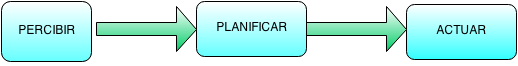
\includegraphics[scale=0.7]{imagenes/jerarquico.png} 
\caption{Paradigma Jer\'arquico}
\label{fig:jerarquico}
\end{figure}


\subsection{Paradigma Reactivo}
El paradigma reactivo omite por completo el componente de la planificación y s\'olo se basa en percibir y actuar. El robot puede mantener un conjunto de pares percibir-actuar como se muestra en la figura \ref{fig:reactivo}, \'estos son llamados comportamientos y se ejecutan como procesos concurrentes. Un comportamiento toma datos de la percepción del mundo y los procesa para tomar la mejor acción independientemente de los otros procesos \cite{AiRobotics}.

\begin{figure}[hbtp]

\centering
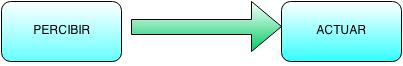
\includegraphics[scale=0.7]{imagenes/reactivo.jpg} 
\caption{Paradigma Reactivo}
\label{fig:reactivo}
\end{figure}


\subsection{Paradigma Híbrido}
El paradigma híbrido es una mezcla de los dos paradigmas anteriores. Primero se planifica cúal es la mejor manera de cumplir el objetivo principal, descomponiendo la tarea general en sub-tareas y decidiendo que comportamientos sirven para cumplir cada una. De allí en adelante se ejecutan los comportamientos (percibiendo y actuando), hasta que el plan sea ejecutado, si es necesario se puede volver a planificar. Vale la pena acotar que la información de los sensores se encuentra disponible para el planificador, de manera que pueda crear un modelo del mundo y tomar decisiones en base a él  \cite{AiRobotics}. 
Se puede apreciar el la figura \ref{fig:hibrido}
\begin{figure}[hbtp]

\centering
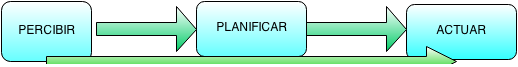
\includegraphics[scale=0.7]{imagenes/hibrido.png} 
\caption{Paradigma H\'ibrido}
\label{fig:hibrido}
\end{figure}
